\chapter{Comunicação Servidor-Cliente}
Para cumprir com os requisitos do enunciado, implementamos um servidor e
um cliente que comunicam via sockets (TCP). 

 A \textit{ServerThread} tem como objectivo receber mensagens por parte do Cliente e  enviar mensagens para o Cliente. Do lado do Cliente verifica-se a mesma estrutura, onde o Cliente envia mensagens e recebe mensagens por parte do Servidor. As mensagens neste problema em questão, são orientadas à linha, isto é a comunicação é feita através de linhas de texto (Strings), onde cada linha de texto equivale a uma mensagem. A imagem que se segue clarifica melhor a estruturação: 
 
\begin{figure}[tbph]
	\centering
	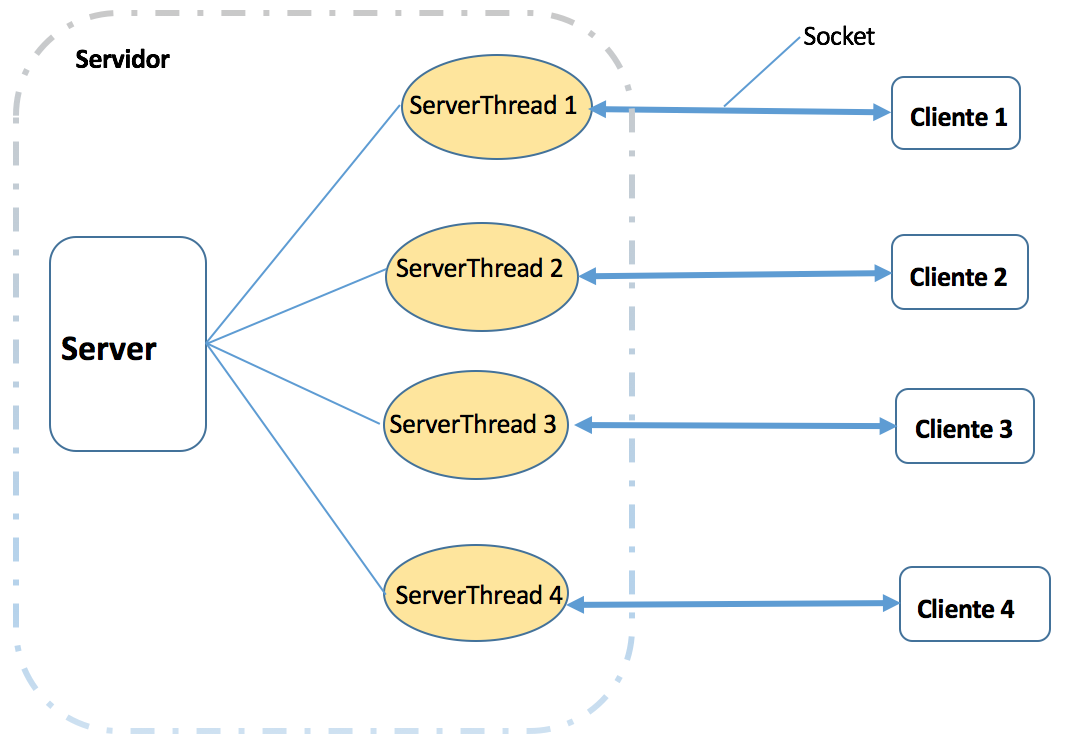
\includegraphics[scale=0.5]{imagem/CominicacaoServidorCliente.png}
	\caption{Comunicação entre cliente e servidor}
	\label{fig:cominicacaoservidorcliente}
\end{figure}
 

\chapter{Controlo de Concorrência}
O principal objectivo deste trabalho é controlar o acesso ao conjunto das threads a zonas criticas da aplicação. Foram identificadas três situações onde o controlo de concorrência seria necessário. 

\section{Formação das equipas}

Cada thread tenta formar uma equipa com jogadores com o mesmo ranking, superior uma unidade ou inferior uma unidade. Se não houverem os 10 jogadores, os existentes que querem jogar serão adicionados a uma lista e o seu estado alterado para \textit{setWaiting(true)}  e ficarão adormecidos numa condição \textit{wantTeamCondition.await()}. 

Se a thread conseguir formar equipa, o estado dos elementos desse jogo é alterado por esta Thread e o estado deixa de ser à espera para formar equipa: \textit{setWaiting(false)} (invocando o método \textit{updateWaitingTeamStatus(team))} que muda o estado de toda a equipa) e de seguida são removidos todos os elementos da lista, pois já não estão à espera de equipa. Após efetuar estas ações a thread que conseguiu formar equipa acorda todas as threads que estavam a dormir (\textit{wantTeamCondition.signalAll();}) porque não tinham conseguido formar equipa. De todas as threads que estavam a dormir nesta condição (não tinham conseguido formar equipa) só irão prosseguir para jogo as que o seu estado (\textit{waiting=false}) foi alterado pela thread que conseguiu formar equipa, todas as outras irão voltar a adormecer.  

A thread que formou equipa para além do descrito acima cria também o objeto \textit{Game} que contém toda a informação do jogo e  invoca a classe \textit{TimeOut} que será a responsável por limitar o tempo de escolha do herói por 30 segundos. 

\subsection{Problemas desta solução}
Um problema desta solução é que se um jogador não conseguir uma equipa com jogadores com ranking semelhante ao dele irá ficar infinitamente à espera de equipa.


\section{Seleção de herói}

Após o utilizador confirmar o seu herói ele irá validar se todos os outros elementos do jogo tem o herói também confirmado, se nem todos tiverem o herói confirmado e se o tempo limite do \textit{timeOut} não tiver chegado ao fim as threads irão adormcer numa fila de espera especifica para os utilizadores que esperam que toda e equipa tenha os herois selecionados. Caso todos os elementos do jogo tenham herói confirmado e o \textit{timeOut} não tiver sido excedido, esta thread irá alterar o estado do jogo \textit{timeout = false}, gera o resultado aleatório do jogo e acorda todas a threads que estão em fila à espera que todos os elementos da equipa tenham herói confirmado (\textit{this.wantGameCondition.signalAll()}). Apesar de acordarmos todas as threads que estão nesta fila só irão prosseguir para jogo as do jogo em questão, todas as outras irão voltar a adormecer. 

\section{Tempo máximo de seleção de herói}

A classe \textit{Timeout} é uma classe que extende Thread e portanto irá ser executada numa outra \textit{thread}, por isso mesmo é que apesar do método \textit{run()} executar um \textit{sleep()} o programa não bloqueia. Após a thread adormecer 30 segundos ela irá tentar alterar o estado do jogo para \textit{timeout==true}, todo o método que tenta alterar o estado do Jogo está dentro do mesmo \textit{ReentrantLock()}), por este motivo a alteração desta variável será executada no máximo por uma thread (sem concorrência) garantimos assim a exclusão mútua nesta seccção critica do código. O estado do Jogo poderá também ser alterado pelo fluxo normal do programa mas o método responsável por efetuar esta acção encontra-se restringido pelo mesmo \textit{ReentrantLock()}) que é usado pelo \textit{Timeout} evitamos assim problemas de concorrência ao aceder/alterar esta variável. 

No caso da classe \textit{Timeout} o método que altera a variável de estado do jogo (só o irá fazer se o fluxo normal ainda não tiver atualizado esta variável e vice-versa). Se conseguir alterar o estado da variável de seguida irá acordar todas as threads que estão adormecidas numa condição em que estão à espera que todos os elementos do jogo tenham o herói confirmado. Desta forma garantimos que quando o tempo limite de escolha de herói é atingido se existirem clientes que estejam adormecidos na fase de escolha de herói são acordados, não necessitamos assim que todos os utilizadores tenham escolhido herói para saberem que o tempo máximo foi excedido. 

\subsection{Problema desta solução}
O problema desta solução é que só depois de os utilizadores confirmarem herói é que irão saber se a partida foi abortada ou não. 
Em suma  o utilizador não sabe em tempo real que o timout aconteceu, apesar disso garantimos que os jogos com mais de 30 segundos na escolha do herói são abortados e não temos threads bloqueantes no fluxo normal do programa ou que fazem esperas ativas.
  
